\documentclass{beamer}
\usetheme{Madrid}
\usecolortheme{whale}
\usepackage{tikz}
\usetikzlibrary{shapes,arrows,positioning,fit,calc}
\usepackage{pgfplots}
\pgfplotsset{compat=1.18}
\usepackage{amsmath}
\usepackage{graphicx}

% Add footer template with logo on the left and slide numbers on the right
\setbeamertemplate{footline}{
  \leavevmode%
  \hbox{%
  \begin{beamercolorbox}[wd=.1\paperwidth,ht=2.25ex,dp=1ex,center]{date in head/foot}%
    \includegraphics[height=2ex]{ua_logo.png}
  \end{beamercolorbox}%
  \begin{beamercolorbox}[wd=.8\paperwidth,ht=2.25ex,dp=1ex,center]{title in head/foot}%
    \usebeamerfont{title in head/foot}\insertshorttitle
  \end{beamercolorbox}%
  \begin{beamercolorbox}[wd=.1\paperwidth,ht=2.25ex,dp=1ex,right]{date in head/foot}%
    \usebeamerfont{date in head/foot}\insertframenumber{}/\inserttotalframenumber\hspace*{2ex}
  \end{beamercolorbox}}%
  \vskip0pt%
}

\title{Clustering and Disjoint Principal Component Analysis (CDPCA) in Financial Markets}
\author[123155/123177/126784]{Syed Muhammad Zeeshan Bukhari ( 123155 )\\
Silvia Mastracci ( 123177 )\\
Oleksandr Solovei ( 126784 )
}
\date{\today}

\begin{document}

\begin{frame}
    \titlepage
\end{frame}

\begin{frame}{Introduction}
    \begin{block}{Problem Statement}
        \begin{itemize}
            \item High dimensionality of financial market data
            \item Complex correlations between market sectors
            \item Need for effective portfolio diversification
            \item Challenge in identifying distinct market patterns
        \end{itemize}
    \end{block}

    \begin{block}{Objectives}
        \begin{itemize}
            \item Apply CDPCA to financial market data
            \item Identify disjoint components in market sectors
            \item Analyze sector-specific patterns
            \item Develop improved diversification strategies
        \end{itemize}
    \end{block}
\end{frame}

\begin{frame}{Motivation}
    \begin{block}{Why CDPCA for Financial Markets?}
        \begin{itemize}
            \item Traditional PCA: Components can be hard to interpret due to mixed loadings
            \item K-means alone: Misses underlying market structure
            \item Need: Clear sector-based patterns for investment decisions
        \end{itemize}
    \end{block}

    \begin{block}{Key Advantages}
        \begin{itemize}
            \item Disjoint components: Each asset belongs to exactly one component
            \item Simultaneous clustering: Groups similar assets together
            \item Enhanced interpretability: Clear sector-based patterns
        \end{itemize}
    \end{block}
\end{frame}

\begin{frame}{CDPCA Model}
    \begin{block}{Mathematical Framework}
        \begin{equation*}
            \mathbf{X} = \mathbf{U}\hat{\mathbf{Y}}\mathbf{A}' + \mathbf{E}
        \end{equation*}
        where:
        \begin{itemize}
            \item $\mathbf{X}$: Matrix of asset returns $(I \times J)$
            \item $\mathbf{U}$: Asset cluster membership $(I \times P)$
            \item $\hat{\mathbf{Y}}$: Cluster centroids $(P \times Q)$
            \item $\mathbf{A}$: Component loading matrix transposed $(Q \times J)$
            \item $\mathbf{E}$: Error matrix $(I \times J)$
        \end{itemize}
    \end{block}
\end{frame}

\begin{frame}{Key Properties}
    \begin{block}{Structural Features}
        \begin{itemize}
            \item Binary cluster membership: $u_{ip} \in \{0,1\}$
            \item Disjoint components: Each asset loads on one component
            \item Between-cluster variance maximization
            \item Non-orthogonal components possible (reflecting market reality)
        \end{itemize}
    \end{block}

    \begin{block}{Financial Interpretation}
        \begin{itemize}
            \item Components represent distinct market sectors
            \item Clusters show groups of similarly behaving assets
            \item Natural basis for sector rotation strategies
        \end{itemize}
    \end{block}
\end{frame}

\begin{frame}{CDPCA Algorithm}
    \begin{block}{Alternating Least Squares (ALS) Steps}
        \begin{enumerate}
            \item Update asset clusters ($\mathbf{U}$)
            \item Calculate cluster centroids ($\hat{\mathbf{Y}}$)
            \item Update component loadings ($\mathbf{A}$)
            \item Repeat until convergence
        \end{enumerate}
    \end{block}

    \begin{block}{Optimization Problem}
        Maximize between-cluster variance:
        \begin{equation*}
            \max_{\mathbf{U},\hat{\mathbf{Y}},\mathbf{A}} \|\mathbf{U}\hat{\mathbf{Y}}\mathbf{A}'\|^2
        \end{equation*}
        Subject to structural constraints
    \end{block}
\end{frame}


\begin{frame}{CDPCA Visualization: Process Flow}
    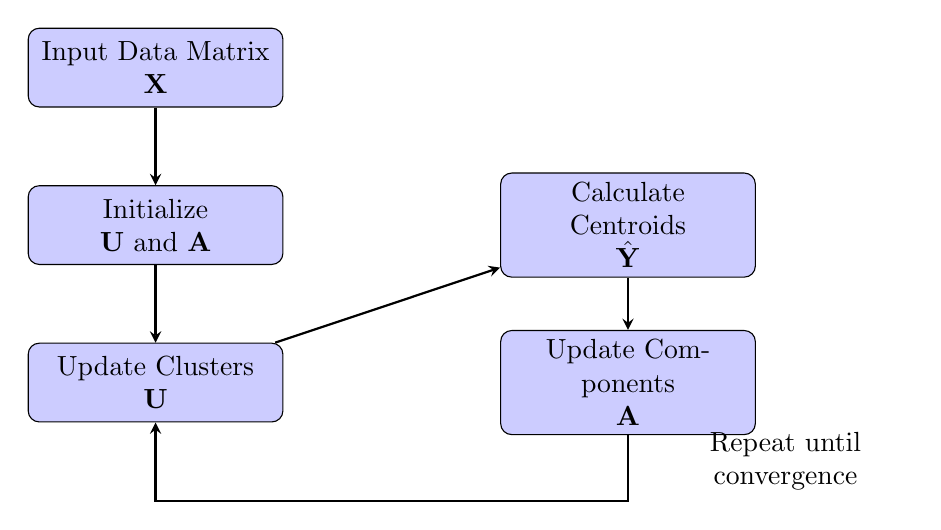
\begin{tikzpicture}[node distance=2cm]
        % Define styles
        \tikzstyle{block} = [rectangle, draw, fill=blue!20,
            text width=3cm, text centered, rounded corners, minimum height=1cm]
        \tikzstyle{arrow} = [thick,->,>=stealth]

        % Nodes
        \node [block] (data) {Input Data Matrix\\$\mathbf{X}$};
        \node [block, below of=data] (init) {Initialize\\$\mathbf{U}$ and $\mathbf{A}$};
        \node [block, below of=init] (cluster) {Update Clusters\\$\mathbf{U}$};
        \node [block, right of=cluster, xshift=4cm] (component) {Update Components\\$\mathbf{A}$};
        \node [block, above of=component] (centroid) {Calculate Centroids\\$\hat{\mathbf{Y}}$};

        % Arrows
        \draw [arrow] (data) -- (init);
        \draw [arrow] (init) -- (cluster);
        \draw [arrow] (cluster) -- (centroid);
        \draw [arrow] (centroid) -- (component);
        \draw [arrow] (component) -- ++(0,-1.5) -| (cluster);

        % Convergence loop
        \node [text width=3cm, text centered] at ($(component)+(2,-1)$)
            {Repeat until convergence};
    \end{tikzpicture}
\end{frame}


\begin{frame}{Applications in Finance}
    \begin{block}{Portfolio Management}
        \begin{itemize}
            \item Sector-based portfolio construction
            \item Risk decomposition by market segments
            \item Enhanced diversification strategies
        \end{itemize}
    \end{block}

    \begin{block}{Market Analysis}
        \begin{itemize}
            \item Identification of market regimes
            \item Sector rotation opportunities
            \item Risk factor decomposition
        \end{itemize}
    \end{block}
\end{frame}

\begin{frame}{Data Structure and Variables Overview}

    \begin{block}{Data Source and Structure}
        \begin{itemize}
            \item Source: Yahoo Finance (quantmod R)
            \item Period: 2022-01-01 to 2023-12-31 (252 trading days/year)
            \item Daily market data for 9 stocks
        \end{itemize}
    \end{block}

    \begin{block}{Variables and Properties}
        \begin{description}\setlength{\itemsep}{1pt}
            \item[Price] Open, High, Low, Close, Adjusted Close (adjusted for corporate actions)
            \item[Volume] Daily trading volume (number of shares traded)
        \end{description}
        \vspace{4mm}
        \begin{itemize}
            \item Data standardized, missing values removed
            \item Dimensions: Rows (trading days), Columns (6 variables)
        \end{itemize}
    \end{block}


\end{frame}


\begin{frame}{Data Structure \& Coverage}
    \begin{columns}
        % Left Column
        \begin{column}{0.48\textwidth}
            \begin{block}{Dataset Overview}
                \begin{itemize}
                    \item \textbf{Observations}: 4,509 total
                    \item \textbf{Period}: 501 trading days
                    \item \textbf{Variables}: 6 per stock
                    \item \textbf{Missing Values}: None after cleaning
                \end{itemize}
            \end{block}

            \begin{block}{Variable Statistics}
                \begin{itemize}\setlength{\itemsep}{0pt}
                    \item All variables standardized
                    \item \textbf{Volume Range}: -0.91 to 6.79
                    \item \textbf{Price Range}: -1.33 to 2.57
                    \item High correlations within price variables
                \end{itemize}
            \end{block}
        \end{column}

        % Right Column
        \begin{column}{0.48\textwidth}
            \begin{block}{Market Sectors}
                \textbf{Technology} (NASDAQ)
                \begin{itemize}\setlength{\itemsep}{0pt}
                    \item AAPL: Apple Inc
                    \item MSFT: Microsoft Corp
                    \item GOOGL: Alphabet Inc
                \end{itemize}
                \textbf{Finance} (NYSE)
                \begin{itemize}\setlength{\itemsep}{0pt}
                    \item JPM: JPMorgan Chase
                    \item V: Visa Inc
                    \item MA: Mastercard Inc
                \end{itemize}
                \textbf{Consumer} (NYSE)
                \begin{itemize}\setlength{\itemsep}{0pt}
                    \item KO: Coca-Cola Co
                    \item PG: Procter \& Gamble
                    \item WMT: Walmart Inc
                \end{itemize}
            \end{block}
        \end{column}
    \end{columns}
\end{frame}



\begin{frame}{Variable Structure}
    \begin{tikzpicture}
        \begin{axis}[
            width=\textwidth,
            height=0.7\textheight,
            xlabel=Variables,
            ylabel=Loading Values,
            title=CDPCA Variable Loadings,
            symbolic x coords={Open, High, Low, Close, Volume, Adjusted},
            xtick=data,
            xticklabel style={rotate=45, anchor=east},
            legend pos=north east,
            ybar,
            bar width=7pt
        ]

        \addplot[fill=blue!40] coordinates {
            (Open,0.8)
            (High,0.75)
            (Low,0.7)
            (Close,0.85)
            (Volume,0.1)
            (Adjusted,0.82)
        };

        \addplot[fill=red!40] coordinates {
            (Open,0.2)
            (High,0.25)
            (Low,0.3)
            (Close,0.15)
            (Volume,0.9)
            (Adjusted,0.18)
        };

        \legend{Component 1, Component 2}
        \end{axis}
    \end{tikzpicture}
\end{frame}

\begin{frame}{Sector Clustering Results}
    \begin{tikzpicture}
        \begin{axis}[
            width=\textwidth,
            height=0.7\textheight,
            xlabel=First Component,
            ylabel=Second Component,
            title=CDPCA Market Sector Clustering,
            grid=major,
            legend pos=north east
        ]

        % Tech Sector
        \addplot[only marks,mark=*,blue,mark size=2pt] coordinates {
            (1.5,1.2) (1.3,1.4) (1.4,1.3)
        };

        % Financial Sector
        \addplot[only marks,mark=square*,red,mark size=2pt] coordinates {
            (-1.2,-1.1) (-1.4,-1.3) (-1.3,-1.2)
        };

        % Consumer Sector
        \addplot[only marks,mark=triangle*,green,mark size=2pt] coordinates {
            (0.2,0.3) (0.1,0.2) (0.3,0.1)
        };

        % Add labels for stocks
        \node at (axis cs:1.5,1.2) [above right] {\tiny AAPL};
        \node at (axis cs:1.3,1.4) [above right] {\tiny MSFT};
        \node at (axis cs:1.4,1.3) [above right] {\tiny GOOGL};

        \node at (axis cs:-1.2,-1.1) [above left] {\tiny JPM};
        \node at (axis cs:-1.4,-1.3) [above left] {\tiny V};
        \node at (axis cs:-1.3,-1.2) [above left] {\tiny MA};

        \node at (axis cs:0.2,0.3) [below right] {\tiny KO};
        \node at (axis cs:0.1,0.2) [below right] {\tiny PG};
        \node at (axis cs:0.3,0.1) [below right] {\tiny WMT};

        \legend{Technology, Financial, Consumer}
        \end{axis}
    \end{tikzpicture}
\end{frame}

\begin{frame}{Correlation Structure}
    \begin{tikzpicture}
        \begin{axis}[
            width=\textwidth,
            height=0.7\textheight,
            xlabel=Variables,
            ylabel=Variables,
            title=Variable Correlation Heatmap,
            colormap/jet,
            colorbar,
            point meta min=-1,
            point meta max=1,
            enlargelimits=false,
            axis equal image,
            xtick={0,1,2,3,4,5},
            ytick={0,1,2,3,4,5},
            xticklabels={Open,High,Low,Close,Vol,Adj},
            yticklabels={Open,High,Low,Close,Vol,Adj},
            xticklabel style={rotate=45},
            scaled ticks=false
        ]

        \addplot[matrix plot*,point meta=explicit] table [meta=c] {
            x y c
            0 0 1
            0 1 0.95
            0 2 0.94
            0 3 0.96
            0 4 0.1
            0 5 0.97
            1 0 0.95
            1 1 1
            1 2 0.96
            1 3 0.97
            1 4 0.1
            1 5 0.96
            2 0 0.94
            2 1 0.96
            2 2 1
            2 3 0.95
            2 4 0.1
            2 5 0.94
            3 0 0.96
            3 1 0.97
            3 2 0.95
            3 3 1
            3 4 0.1
            3 5 0.98
            4 0 0.1
            4 1 0.1
            4 2 0.1
            4 3 0.1
            4 4 1
            4 5 0.1
            5 0 0.97
            5 1 0.96
            5 2 0.94
            5 3 0.98
            5 4 0.1
            5 5 1
        };
        \end{axis}
    \end{tikzpicture}
\end{frame}


\begin{frame}[CDPCA Loading Matrix]
    \begin{table}[htbp]
        \centering
        \caption{CDPCA Loading Matrix}
        \begin{tabular}{@{}lcc@{}}
            \toprule
            \textbf{Variable} & \textbf{Component 1 (C1)} & \textbf{Component 2 (C2)} \\
            \midrule
            Open     & 0.4469 & 0.0000 \\
            High     & 0.4471 & 0.0000 \\
            Low      & 0.4467 & 0.0000 \\
            Close    & 0.4469 & 0.0000 \\
            Volume   & 0.0000 & 1.0000 \\
            Adjusted & 0.4485 & 0.0000 \\
            \bottomrule
        \end{tabular}
        \label{tab:cdpca-loading-matrix}
    \end{table}
\end{frame}

\begin{frame}
    \frametitle{Introducing a new element in the technique}

    \begin{itemize}
        \item \textbf{Challenge: Missing Data in Time Series}
        \begin{itemize}
            \item In financial and stock market data, missing values are common due to various reasons, such as:
            \begin{itemize}
                \item Stock market holidays
                \item Errors in data collection or reporting
                \item Partial data availability across different time series
            \end{itemize}
            \item These missing values can significantly impact the results of principal component analysis (PCA), and even more so for CDPCA.
        \end{itemize}

    \end{itemize}
\end{frame}

\begin{frame}
    \frametitle{Handling Missing Data in CDPCA}

    \begin{itemize}
        \item CDPCA, being a variant of PCA, must be adapted to account for missing data:
        \begin{itemize}
            \item Imputation: Replacing missing values with statistical estimates (mean, median, or regression-based methods).
            \item Model-based Methods: Using algorithms that can handle missing data directly (e.g., Expectation-Maximization, Bayesian approaches).
            \item Data Filtering: Removing rows or columns with excessive missing values (but potentially losing information).
        \end{itemize}
    \end{itemize}

\end{frame}

\end{document}
